\documentclass{article}
\usepackage{spalign}
\usepackage{graphicx}
\usepackage{amsmath}
\usepackage{amsfonts}
\usepackage{xcolor}

\title{Choose Your Calculus Adventure \\
        Diagnostic Questions}
\author{John Guzauckas}
\date{\today}

\begin{document}
\maketitle

\section{Algebra Problems}
\begin{enumerate}
\item What is the slope of the line through the points $(3, -5)$ and $(1, -1)$?

\[(3, -5) = (x_{1},y_{1}), (1, -1) = (x_{2}, y_{2})\]
\[m = \frac{y_{2}-y_{1}}{x_{2}-x_{1}} = \frac{-1 - (-5)}{1 - 3} = \frac{4}{-2} = -2\]

The slope of the line through is the points $(3, -5)$ and $(1, -1)$ is $-2$.

\item The lines $3x + 2y = 7$ and $x - 3y = 6$ intersect at a point with what coordinates?

\[3x + 2y = 7 \Longrightarrow 3x = 7 - 2y \Longrightarrow x = \frac{7 - 2y}{3}\]
\[x - 3y = 6 \Longrightarrow \frac{7 - 2y}{3} - 3y = 6 \]
\[\Longrightarrow 7 - 2y - 9y = 18 \Longrightarrow -11y = 11 \Longrightarrow y = -1\]
\[x = \frac{7 - 2y}{3} \Longrightarrow x = \frac{7 - 2(-1)}{3} \Longrightarrow \frac{7 + 2}{3}
\Longrightarrow x = \frac{9}{3} \Longrightarrow x = 3\]

The lines $3x + 2y = 7$ and $x - 3y = 6$ intersect at the point $(3, -1)$

\item Which of the following expressions is equivalent to ${\left(\frac{1}{x} + \frac{1}{y}\right)}^{-1}$?
    \begin{enumerate}
    \item $x - y$
    \item $x + y$
    \item $x^{2} + y^{2}$
    \item $\frac{1}{x} + \frac{1}{y}$
    \item $\frac{1}{x^{2}} + \frac{1}{y^{2}}$
    \item $\frac{xy}{x + y}$
    \item $\frac{x + y}{xy}$
    \item None of the above
    \end{enumerate}
\[{\left(\frac{1}{x} + \frac{1}{y}\right)}^{-1} \Longrightarrow 
    {\left(\frac{y}{xy} + \frac{x}{xy}\right)}^{-1} \Longrightarrow
    {\left(\frac{y + x}{xy}\right)}^{-1} \Longrightarrow
    \frac{xy}{x + y}\] 

So ${\left(\frac{1}{x} + \frac{1}{y}\right)}^{-1}$ is equivalent to (f) $\frac{xy}{x + y}$.

\item List all possible solutions to the equation $x^{3} - x^{2} - 2x = 0$.

\[x^{3} - x^{2} - 2x = 0 \Longrightarrow x(x^{2} - x - 2) = 0 \Longrightarrow x(x + 1)(x - 2) = 0\]
\[x = 0\]
\[x + 1 = 0 \Longrightarrow x = -1\]
\[x - 2 = 0 \Longrightarrow x = 2\]
So the possible solutions to $x^{3} - x^{2} - 2x = 0$ are $-1, 0, 2$.

\item A $0.25$mL sample of water drawn from a $5$ liter flask contains $1.25\times 10^{8}$ bacteria.
Give the approximate number of bacteria in the flask, expressing your answer in scientific notation.

$5$ liters is the same as $5000$mL. We can find our multiplier by dividing the total volume by the sample volume.
\[x = \frac{5000}{0.25} \Longrightarrow x = 20000\]
\[1.25 \times 10^{8} \times 20000 \Longrightarrow 1.25 \times 10^{8} \times 2 \times 10^{4}\]
\[\Longrightarrow 1.25 \times 2 \times 10^{8} \times 10^{4} \Longrightarrow 2.5 \times 10^{12}\]

The total number of bacteria in the flask is approximately $2.5 \times 10^{12}$.

\item For what value of the constant $a$ will the following system of linear equations have no solution?
\spalignsysdelims..
\[
  \spalignsys{
    6x - 5y = 3;
    3x + ay = 1
  }
\]

A system of linear equations will have no solutions given they have the same slope but different y-intercepts.
\[6x - 5y = 3 \Longrightarrow -5y = 3 - 6x \Longrightarrow y = \frac{6}{5}x - \frac{3}{5}\]
\[3x + ay = 1 \Longrightarrow ay = 1 - 3x \Longrightarrow y = \frac{-3}{a}x + \frac{1}{a}\]
So $m_{1} = \frac{6}{5}$ and $m_{2} = \frac{-3}{a}$.
\[m_{1} = m_{2} \Longrightarrow \frac{6}{5} = \frac{-3}{a} \Longrightarrow 6a = -15 \Longrightarrow a = -2.5\]
We also know that the y-intercepts cannot be equal.
\[\frac{3}{5} \neq \frac{1}{-2.5} \Longrightarrow -7.5 \neq 5 \checkmark\]
So the constant $a = -2.5$ will result in the system having no solutions.

\item Find the value of the constant $a$ for which the polynomial $x^{3} + ax^{2} - 1$ will have $-1$ as a root.

\[{(-1)}^{3} + a{(-1)}^{2} - 1 = 0 \Longrightarrow -1 + a - 1 = 0 \Longrightarrow a - 2 = 0 \Longrightarrow a = 2\]
When $a = 2$, the polynomial will have $-1$ as a root.

\item If $a_{n} = \frac{x^{n}}{2^{n}n!}$, find $\frac{a_{n + 1}}{a_{n}}$.
    \begin{enumerate}
    \item $\frac{x^{n + 1}}{2^{n + 1}(n + 1)}$!
    \item $\frac{nx^{n}}{2^{n}(n + 1)}$
    \item $\frac{nx}{2^{n}(n + 1)}$
    \item $\frac{x}{2^{n}(n + 1)}$
    \item $\frac{x}{2(n + 1)}$
    \end{enumerate}

\[\frac{a_{n + 1}}{a_{n}} \Longrightarrow \frac{\frac{x^{n + 1}}{2^{n + 1}(n + 1)!}}{\frac{x^{n}}{2^{n}n!}}
    \Longrightarrow \frac{x^{n + 1}}{2^{n + 1}(n + 1)!}\times\frac{2^{n}n!}{x^{n}}
    \Longrightarrow \frac{x^{n + 1}2^{n}n!}{x^{n}2^{n + 1}(n + 1)!}\]
\[\Longrightarrow \frac{x^{n}x2^{n}n!}{x^{n}2^{n}2(n + 1)n!}
    \Longrightarrow \frac{x}{2(n + 1)}\]
$\frac{a_{n + 1}}{a_{n}}$ is equivalent to (e) $\frac{x}{2(n + 1)}$.
\end{enumerate}

\pagebreak
\section{Geometry Problems}
\begin{enumerate}
\item A bed that is $4$ feet wide must enter through a door (that is just over $4$\\
feet wide) along the $8$ foot wall of a $8$ by $20$ foot room. What is the largest\\
length of a bed that can be rotated to fit with the longest side along the $8$\\
foot long wall opposite the door?
\\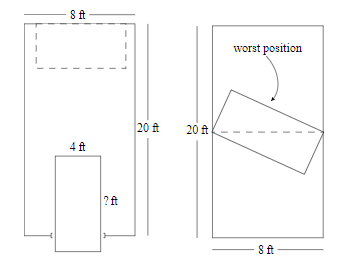
\includegraphics[scale=1]{Images/Geo1.png}

According to the Pythagorean Theorem, the diagonal length of the bed must be the
sum of the squares of its length and width.
We know the width of the bed is $4$ feet and the diagonal needs to stop at $8$ feet.
\[4^{2} + l^{2} = 8^{2} \Longrightarrow l^{2} = 64 - 16 \Longrightarrow l^{2} = 48
    \Longrightarrow l = \sqrt{48} \Longrightarrow l = 2\sqrt{12}\]

The largest length of a bed is $l = 2\sqrt{12} \approx 6.93$ feet

\pagebreak
\item The four-sided solid shown was the part of the solid sphere (of radius 2,\\
centered at the origin) in the first octant. Find its total surface area.
\\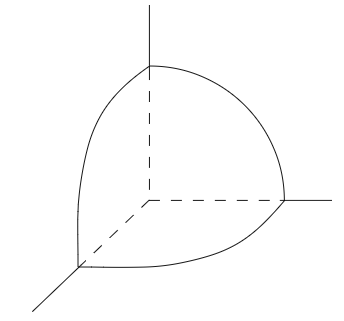
\includegraphics[scale = 1]{Images/Geo2.png}

To find the surface area, we find the area of each of the four sides of the solid.
The outer curved side is an eighth of the total surface area for a sphere.
The inner walls are each one quarter of the area of a circle with the same radius as the sphere,
which with three sides, makes three quarters of the area of the circle.
\[SA = \frac{1}{8}\times 4\pi r^{2} + \frac{3}{4}\pi r^2
    \Longrightarrow SA = \frac{1}{2}\pi {(2)}^{2} + \frac{3}{4}\pi {(2)}^{2}\]
\[\Longrightarrow SA = \frac{1}{2}\times 4\pi + \frac{3}{4}\times 4\pi
    \Longrightarrow SA = 2\pi + 3\pi \Longrightarrow SA = 5\pi\]
The surface area of the first octant of this sphere is $5\pi$.

\pagebreak
\item To estimate the height of a skyscraper $1$km in the distance, Jenny finds\\
that if her friend Steve stands $2.5$ meters away, the top of his head just\\
lines up with the topc of the building. Steve is $2$ meters tall, and Jenny's\\
eye is $1.5$ meters from the ground. How high is the building?
\\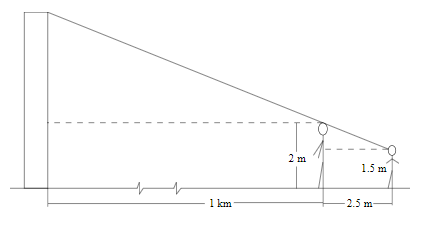
\includegraphics[scale = 0.95]{Images/Geo3.png}

To calculate the height, we need to calculate the height of the triangle made by Steve's
head and the building. We know the length of the base of the triangle is $1$km, but
we need additional information in order to calculate the height. To do this, we can use
the triangle between Jenny and Steve, as it is similar to the larger triangle. In similar
triangles, the ratios of corresponding sides must remain constant. To calculate the ratio,
we can use the lengths of the bases of the similar triangles.
\[r = \frac{1000}{2.5} \Longrightarrow r = 400\]
Now we can set up a ratio using the heights of the similar triangles
\[400 = \frac{h}{0.5} \Longrightarrow h = 200\]
This is not the final height of the building, as we have not accounted for Steve's height yet.
\[h = 200 + 2 \Longrightarrow h = 202\]
The height of the building is 202 meters.
\end{enumerate}

\section{Trigonometry}
\begin{enumerate}
\item In the given right triangle, what is $\tan(y)$?
\\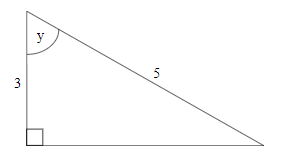
\includegraphics[scale = 1]{Images/Trig1.png}

\[\tan(y) = \frac{\text{opposite}}{\text{adjacent}}\]
In the given triangle, we know the adjacent side and the hypotenuse, so we must calculate
the opposite side using the pythagorean theorem.
\[a^{2} + b^{2} = c^{2} \Longrightarrow 3^{2} + b^{2} = 5^{2} \Longrightarrow b^{2} = 16
    \Longrightarrow \sqrt{b^{2}} = \sqrt{16} \Longrightarrow b = 4\]
\[\tan(y) = \frac{\text{opposite}}{\text{adjacent}} \Longrightarrow \tan(y) = \frac{4}{3}\]
For this right triangle, $\tan(y) = \frac{4}{3} \approx 1.33$.

\pagebreak
\item A horse runs counterclockwise (anticlockwise) around the circular track of radius $400$m
a constant speed, starting at the marked point. It completes one lap in three minutes. What is
its y-coordinate after one minute?
\\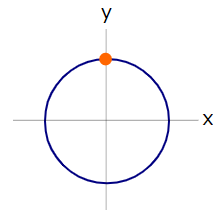
\includegraphics[scale = 1]{Images/Trig2.png}

The horse completes one lap in three minutes, which means in one minute, it completes
one-third of a lap.
\[\theta = \frac{1}{3}\times 2\pi + \frac{\pi}{2}
    \Longrightarrow \theta = \frac{2\pi}{3} + \frac{\pi}{2}\]
\[\Longrightarrow \theta = \frac{4\pi + 3\pi}{6}
    \Longrightarrow \theta = \frac{7\pi}{6}\]

On a unit circle, the coordinate associated with the angle $\frac{7\pi}{6}$
is \\$\left(-\frac{\sqrt{3}}{2},-\frac{1}{2},\right)$.
To scale our y-coordinate, we multiply by the radius
\[y = 400 \times -\frac{1}{2} \Longrightarrow y = -200\]
The y-coordinate of the horse after one minute is $y = -200$.\

\pagebreak
\item Find the smallest possible solution to the equation $\sin(2x) = \frac{1}{2}$;
here $x$ is in radians.

\[\sin(2x) = \frac{1}{2} \Longrightarrow \sin^{-1}(\sin(2x)) = \sin^{-1}\left(\frac{1}{2}\right)\]
The smallest value for $\sin^{-1}\left(\frac{1}{2}\right)$ is $\frac{\pi}{6}$.
\[2x = \frac{\pi}{6} \Longrightarrow x = \frac{\pi}{12}\]
The smallest possible solution to $\sin(2x) = \frac{1}{2}$ is $x = \frac{\pi}{12}$.

\item A line with slope $\frac{1}{2}$ makes an acute angle $\theta$ with the $x$ axis.
What is $\sin(\theta)$?

A line with a slope of $\frac{1}{2}$ makes a right-triangle with a vertical line at $x = 2$.
The created triangle has a length of 2 and a height of 1.
\[\sin(\theta) = \frac{\text{opposite}}{\text{hypotenuse}}\]
We currently know that the opposite side of our triangle is the height of 1, but we need
to calculate the hypotenuse using the pythagorean theorem.
\[a^{2} + b^{2} = c^{2} \Longrightarrow 1^{2} + 2^{2} = c^{2} \Longrightarrow c^{2} = 5
    \sqrt{c^{2}} = \sqrt{5} \Longrightarrow c = \sqrt{5}\]
\[\sin(\theta) = \frac{\text{opposite}}{\text{hypotenuse}}
    \Longrightarrow \sin(\theta) = \frac{1}{\sqrt{5}}\]
\[\Longrightarrow \sin(\theta) = \frac{1}{\sqrt{5}}\times\frac{\sqrt{5}}{\sqrt{5}}
    \Longrightarrow \sin(\theta) = \frac{\sqrt{5}}{5}\]
Given the line creating $\theta$, $\sin(\theta) = \frac{\sqrt{5}}{5}$

\item By using the trigonometric identity $\cos(2x) = \cos^{2}(x) - \sin^{2}(x)$, and
other identities, find the positive expression for $\sin\left(\frac{A}{2}\right)$ in
terms of $\cos(A)$.

We know that $\cos^{2}(A) = 1 - \sin^{2}(A)$.
\[\cos(2A) = 1 - \sin^{2}(A) - \sin^{2}(A) \Longrightarrow \cos(2A) = 1 - 2\sin^{2}(A)\]

Next step is to divide the input angle by 2, resulting in
\[\cos(A) = 1 - 2\sin^{2}\left(\frac{A}{2}\right)
    \Longrightarrow \cos(A) - 1 = - 2\sin^{2}\left(\frac{A}{2}\right)\]
\[\Longrightarrow \frac{1 - \cos(A)}{2} = \sin^{2}\left(\frac{A}{2}\right)
    \Longrightarrow \sqrt{\frac{1 - \cos(A)}{2}} = \sqrt{\sin^{2}\left(\frac{A}{2}\right)}\]
\[\Longrightarrow \sin\left(\frac{A}{2}\right) = \sqrt{\frac{1 - \cos(A)}{2}}\]
Using the trigonometric identities, we know $\sin\left(\frac{A}{2}\right) = \sqrt{\frac{1 - \cos(A)}{2}}$

\item The graph below represents which of the these functions?
\\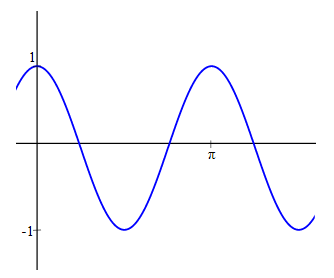
\includegraphics[scale = 1]{Images/Trig3.png}

    \begin{enumerate}
        \item $\sin(x)$
        \item $\cos(x)$
        \item $\sin\left(\frac{x}{2}\right)$
        \item $\cos\left(\frac{x}{2}\right)$
        \item $\sin(2x)$
        \item $\cos(2x)$
    \end{enumerate}

Looking at the graph, we can see that it is a $\cos$ function that has not been vertically
or horizontally shifted, which limits our options to (b), (d), and (f).

We can see that the period of the $\cos$ function has been modified (shrunk), which eliminates
option (b).

A shrinking period is a result of a scale increase of the input, which means that the correct
function is (f) $\cos(2x)$.
\end{enumerate}

\pagebreak
\section{Logarithms and Exponentials}
\begin{enumerate}
\item If $\log_{10}(a) = 4.2$ and $\log_{10}(b) = 0.5$, what is $\log_{10}(ab)$?

\[\log_{10}(ab) = \log_{10}(a) + \log_{10}(b) \Longrightarrow \log_{10}(ab) = 4.2 + 0.5
    \log_{10}(ab) = 4.7\]

\item If $2^{a} = \frac{\sqrt(8)}{4^{3}}$, what is $a$?

\[2^{a} = \frac{\sqrt(8)}{4^{3}}
    \Longrightarrow 2^{a} = \frac{{\left(2^{3}\right)}^{\frac{1}{2}}}{{\left(2^{2}\right)}^{3}}
    \Longrightarrow 2^{a} = \frac{2^{\frac{3}{2}}}{2^{6}}
    \Longrightarrow 2^{a} = 2^{\frac{3}{2}-6}
    \Longrightarrow 2^{a} = 2^{-\frac{9}{2}}\]
\[\Longrightarrow \log_{2}\left(2^{a}\right) = \log_{2}\left(2^{-\frac{9}{2}}\right)
    \Longrightarrow a = -\frac{9}{2} \Longrightarrow a = -4.5\]

\item Which of the following is equal to $\sqrt{\frac{x^{16}(1 + x^{2})}{9}}$?

    \begin{enumerate}
        \item $\frac{x^{4}(1 + x)}{3}$
        \item $\frac{x^{8}(1 + x)}{3}$
        \item $\frac{x^{4}{(1 + x^{2})}^{0.5}}{3}$
        \item $\frac{x^{8}{(1 + x^{2})}^{0.5}}{3}$
        \item $\frac{x^{4}(1 + x^{2})}{3}$
        \item $\frac{x^{8}(1 + x^{2})}{3}$
        \item None of the above
    \end{enumerate}

\[\sqrt{\frac{x^{16}(1 + x^{2})}{9}} \Longrightarrow {\left(\frac{x^{16}(1 + x^{2})}{9}\right)}^{\frac{1}{2}}
    \Longrightarrow \frac{x^{16\times\frac{1}{2}}{(1 + x^{2})}^{\frac{1}{2}}}{3^{2\times\frac{1}{2}}}\]
\[\Longrightarrow \frac{x^{8}{(1 + x^{2})}^{0.5}}{3}\]

$\sqrt{\frac{x^{16}{(1 + x^{2})}}{9}}$ is equivalent to (d) $\frac{x^{8}{(1 + x^{2})}^{0.5}}{3}$

\item Solve for $x$: $\log_{10}\left[{(x + 1)}^{2}\right]=2$

\[\log_{10}\left[{(x + 1)}^{2}\right]=2 \Longrightarrow 2\log_{10}\left[x + 1\right] = 2
    \Longrightarrow \log_{10}\left[x + 1\right] = 1\]
\[\Longrightarrow 10^{\log_{10}\left[x + 1\right]} = 10^{1}
    \Longrightarrow \pm(x + 1) = 10\]
\[\Longrightarrow -x - 1 = 10 \Longrightarrow -x = 11 \Longrightarrow x = -11\]
\[\Longrightarrow x + 1 = 10 \Longrightarrow x = 9\]

\item A pot of water (at sea level) is boiling; the heat is turned off at time $t = 0$,
and $2$ minutes later the water temperature has fallen to $80\circ$C. If the temperature
$T$ (in $\circ$C) is expressed in terms of time $t$ (in minutes) by the law $T = Ae^{-kt}$
Find the values of the constants $A$ and $k$.

So we know $T = 100$ when $t = 0$ and $T = 80$ when $t = 2$.
\[100 = Ae^{-k\times 0} \Longrightarrow 100 = Ae^{0} \Longrightarrow A = 100\]
\[80 = 100e^{-2k} \Longrightarrow 0.8 = e^{-2k} \Longrightarrow \ln(0.8) = \ln\left(e^{-2k}\right)\]
\[\Longrightarrow \ln(0.8) = -2k \Longrightarrow k = -\frac{\ln(0.8)}{2}\]

So we know $A = 100$ and $k = -\frac{\ln(0.8)}{2} \approx 0.11$.
\end{enumerate}
\end{document}